\documentclass{article}

\usepackage{fancyhdr}
\usepackage{extramarks}
\usepackage{amsmath}
\usepackage{amsthm}
\usepackage{amsfonts}
\usepackage{tikz}
\usepackage[plain]{algorithm}
\usepackage{algpseudocode}
\usepackage{enumerate}
\usepackage{mathrsfs}
\usepackage{bm}
\usepackage{amssymb}
\usepackage{tikz}  
\usetikzlibrary{arrows.meta}
\usetikzlibrary{automata,positioning}

%
% Basic Document Settings
%  

\topmargin=-0.45in
\evensidemargin=0in
\oddsidemargin=0in
\textwidth=6.5in
\textheight=9.0in
\headsep=0.25in

\linespread{1.1}

\pagestyle{fancy}
\lhead{\hmwkAuthorName}
\rhead{\hmwkClass\ (\hmwkClassInstructor): \hmwkTitle}
\cfoot{\thepage}

\renewcommand\headrulewidth{0.4pt}
\renewcommand\footrulewidth{0.4pt}

\setlength\parindent{2em}

%
% Create Problem Sections
%


% \setcounter{secnumdepth}{0}
% \newcounter{partCounter}
% \newcounter{homeworkProblemCounter}
% \setcounter{homeworkProblemCounter}{1}


\newcommand{\hmwkTitle}{Homework II}
\newcommand{\hmwkDueDate}{Oct 26th, 2022}
\newcommand{\hmwkClass}{Introduction to Machine Learing}
\newcommand{\hmwkClassInstructor}{Professor Ziping Zhao}
\newcommand{\hmwkAuthorName}{Bingnan Li}
\newcommand{\hmwkAuthorID}{2020533092}

%
% Title Page
%

\title{
    \vspace{2in}
    \textmd{\textbf{\hmwkClass:\\ \hmwkTitle}}\\
    \normalsize\vspace{0.1in}\small{Due\ on\ \hmwkDueDate\ at 11:59pm}\\
    \vspace{0.1in}\large{\textit{\hmwkClassInstructor}}
    \vspace{3in}
}

\author{\textbf{\hmwkAuthorName}\\ \hmwkAuthorID}
\date{}

% \renewcommand{\part}[1]{\textbf{\large Part \Alph{partCounter}}\stepcounter{partCounter}\\}

%
% Various Helper Commands
%

% Useful for algorithms
\newcommand{\alg}[1]{\textsc{\bfseries \footnotesize #1}}

% For derivatives
\newcommand{\deriv}[1]{\frac{\mathrm{d}}{\mathrm{d}x} (#1)}

% For partial derivatives
\newcommand{\pderiv}[2]{\frac{\partial}{\partial #1} (#2)}

% Integral dx
\newcommand{\dx}{\mathrm{d}x}

% Alias for the Solution section header
\newcommand{\solution}{\textbf{\large Solution}}

% Probability commands: Expectation, Variance, Covariance, Bias
\newcommand{\E}{\mathbb{E}}
\newcommand{\Var}{\mathrm{Var}}
\newcommand{\Cov}{\mathrm{Cov}}
\newcommand{\Bias}{\mathrm{Bias}}
\renewcommand{\b}[1]{\bm{#1}}
\begin{document}

\maketitle
\pagebreak

\begin{enumerate}
    \setlength\parindent{2em}
    \item [1.] [Bayesian Decision Theory]
    \begin{enumerate}
        \setlength\parindent{2em}
        \item [(a)] Specify decision rule via likelihood and posterior respectively, and give example with $x=light$ to use the rules.\newline
        {\bf Solution:}
        \par Likelihood decision rule:
        \begin{align*}
            choose\left\{\begin{aligned}
                C=C_1,&\ if\ P(x|C_1) > P(x|C_2)\\
                C=C_2,&\ elsewhere
            \end{aligned}\right.
        \end{align*}
        \par Posterior decision rule:
        \begin{align*}
            choose\left\{\begin{aligned}
                C=C_1,&\ if\ P(C_1|x) > P(C_2|x)\\
                C=C_2,&\ elsewhere
            \end{aligned}\right.
        \end{align*}
        \par If $x=light$, then likelihood is 
        \[P(x=light|C_1)=\frac{2125}{2125+6375}=0.25\]
        \[P(x=light|C_2)=\frac{1000}{1000+500}=0.667\]
        Thus, by likelihood decision rule, we choose $C_2$.
        However, the posterior probability is
        \[P(C_1|x=light)=\frac{2125}{2125+1000}=0.68\]
        \[P(C_2|x=light)=\frac{1000}{2125+1000}=0.32\]
        Thus, by posterior decision rule, we choose $C_1$.
        \item [(b)]
        \begin{enumerate}
            \setlength\parindent{2em}
            \item [(i)] Find the optimal decision rule that will give the minimum expected loss.\newline
            {\bf Solution:}
            \par Let action $\alpha_i$ be classifying input $\b{x}$ into class $i$ and $R(\alpha_i|\b{x})$ be the expected loss of taking action $\alpha_i$, then we have
            \begin{align*}
                R(\alpha_i|\b{x}) = \sum_{j=1}^K \lambda_{i,j}P(C_k|\b{x})
            \end{align*}
            Then the optimal decision rule is 
            \begin{align*}
                \left\{\begin{aligned}
                    &choose\ class\ i,\ &if\ R(\alpha_i|\b{x})=\min\{R(\alpha_j|\b{x})\}_{j=1}^K < \lambda\\
                    &reject\ \b{x},\ &if\ R(\alpha_i|\b{x})=\min\{R(\alpha_j|\b{x})\}_{j=1}^K \geq \lambda
                \end{aligned}\right.
            \end{align*}
            \item [(ii)] State the relationship between $\lambda$ and the rejection
            threshold $\theta$.\newline
            {\bf Solution:}
            \par Given that $\lambda_{i,k}=\left\{\begin{aligned}
                &1,\ &if\ i\neq k\\
                &0,\ &if\ i=k
            \end{aligned}\right.$
            Then the corresponding expected loss is as following
            \begin{align*}
                R(\alpha_i|\b{x})=\sum_{j=1}^K \lambda_{i,j}P(C_k|\b{x}) = 1-P(C_i|\b{x})
            \end{align*}
            \par In order to get minimum expected loss, we hope:
            \begin{itemize}
                \setlength\parindent{2em}
                \item When $P(C_i|\b{x})>\theta$, we hope that $R(\alpha_i|\b{x})=\min\{R(\alpha_j|\b{x})\}_{j=1}^K= 1-P(C_i|\b{x})\leq \lambda$ so that we won't get expected loss any lower by manually choosing to reject $\b{x}$.
                \par In order to achieve that, we need: 
                \[\lambda\geq max(1-P(C_i|\b{x}))=1-\theta\]
                \item When $P(C_i|\b{x})\leq\theta$, we hope that $\lambda \leq R(\alpha_i|\b{x})=\min\{R(\alpha_j|\b{x})\}_{j=1}^K= 1-P(C_i|\b{x})$ so that we won't get expected loss any lower by selecting to classifying $\b{x}$ into class $i$.
                \par In order to achieve that, we need 
                \[\lambda \leq min(1-P(C_i|\b{x}))=1-\theta\]
            \end{itemize}
            Based on that, we have 
            \begin{align*}
                \lambda &\geq 1-\theta\\
                \lambda &\leq 1-\theta
            \end{align*}
            Therefore, we have 
            \[\lambda = 1-\theta\Rightarrow \lambda + \theta = 1\]
        \end{enumerate}
    \end{enumerate}
    \item [2.] [Parameter Estimation]
    \begin{enumerate}
        \setlength\parindent{2em}
        \item [(a)] Let $\b{X} = [\b{x}_1,\cdots,\b{x}_n]^T$ and $\b{y} = [y_1, \cdots, y_n]^T$. Assume that $e_i\sim \mathcal{N}(0,\sigma^2)$ and $\b{X^TX}$ is a full-rank matrix. Derive the maximum likelihood estimate $\b{w}_{ML} = (\b{X^TX}^{-1}\b{X^Ty})$.\newline
        {\bf Proof:} 
        \par Given that $e_i\sim\mathcal{N}(0,\sigma^2)$ and $y_i = \b{w^Tx_i}+e_i$, we have that 
        \[y_i\sim\mathcal{N}(\b{w^Tx_i}, \sigma^2)\]
        Thus, the likelihood function is
        \begin{align*}
            \mathcal{L}(\b{w}) &= \log(P(\b{y|X,w})) =  -\sum_{i=1}^n\left(\log\sqrt{2\pi}\sigma + \frac{\left(y_i-\b{w^Tx_i}\right)^2}{2\sigma^2}\right)\\
            &= -n\log\sqrt{2\pi}\sigma - \frac{\sum_{i=1}^n\left(y_i-\b{w^Tx_i}\right)^2}{2\sigma^2}\\
            &= -n\log\sqrt{2\pi}\sigma - \frac{||\b{y-Xw}||_2^2}{2\sigma^2}\\
            \frac{\partial\mathcal{L}}{\partial \b{w}} &= -\frac{1}{2\sigma^2} \frac{\partial \b{w^TX^TXw-2w^TX^Ty+y^Ty}}{\partial \b{w}}\\
            &= -\frac{1}{2\sigma^2}\left(2\b{X^TXw}-2\b{X^Ty}\right) = 0\\
            &\Rightarrow \b{X^TXw} = \b{X^Ty}\\
            &\Rightarrow \b{w}_{ML} = \left(\b{X^TX}\right)^{-1}\b{X^Ty}
        \end{align*}
        \item [(b)] Assume $\b{w}\sim\mathcal{N}(0,\nu^2\b{I})$. Derive the maximum a posteriori estimate \[\b{w}_{MAP} = \left(\b{X^TX}+\frac{\sigma^2}{\nu^2}\b{I}\right)^{-1}\b{X^Ty}\]
        {\bf Proof:}
        \par Given that $\b{w}\sim\mathcal{N}(\b{0},\nu^2\b{I})$, we know that 
        \[P(\b{w}) = \frac{1}{(2\pi)^{n/2}\nu}\exp[-\frac{1}{2}(\b{w^T}\frac{1}{\nu^2}\b{I}\b{w})] = \frac{1}{(2\pi)^{n/2}\nu} \exp\left(-\frac{\b{w^Tw}}{2\nu^2}\right)\]
        Then by definition, we know that 
        \begin{align*}
            \b{w}_{MAP} &= \arg\max\limits_{\b{w}} P(\b{w}|\mathcal{D})\\
            &= \arg\max\limits_{\b{w}} \frac{P(\mathcal{D}|\b{w})P(\b{w})}{P(\mathcal{D})}\\
            &= \arg\max\limits_{\b{w}} P(\b{y,X|w})P(\b{w})\\
            &= \arg\max\limits_{\b{w}} P(\b{y|X,w})P(\b{X|w})P(\b{w})
        \end{align*}
        Since the value of $\b{X}$ does not rely on $\b{w}$, we have $P(\b{X|w}) = P(\b{X})$. Sequentially, we have
        \[\b{w}_{MAP} = \arg\max\limits_{\b{w}} P(\b{y|X,w})P(\b{X})P(\b{w}) = \arg\max\limits_{\b{w}} P(\b{y|X,w})P(\b{w})\] 
        \par Next, let $\mathcal{L}(\b{w}) = \log{P(\b{y|X,w})P(\b{w})} = \log{P(\b{y|X,w})}+\log{P(\b{w})}$, we have
        \begin{align*}
            \mathcal{L}(\b{w}) &= -n\log\sqrt{2\pi}\sigma - \frac{||\b{y-Xw}||_2^2}{2\sigma^2} + \log{(2\pi)^{n/2}\nu}-\frac{\b{w^Tw}}{2\nu^2}\\
            \frac{\partial \mathcal{L}}{\partial \b{w}} &= -\frac{\b{X^TXw-X^Ty}}{\sigma^2}-\frac{\b{w}}{\nu^2} = 0\\
            &\Rightarrow \left(\b{X^TX}+\frac{\sigma^2}{\nu^2}\b{I}\right)\b{w} = \b{X^Ty}
        \end{align*}
        Given that $\b{X^TX}$ is full-rank and $\frac{\sigma^2}{\nu^2}\b{I}$ is positive-definite, we know that $\b{X^TX}+\frac{\sigma^2}{\nu^2}\b{I}$ is invertible.
        \par Therefore, we know that
        \[\b{w}_{MAP} = \left(\b{X^TX}+\frac{\sigma^2}{\nu^2}\b{I}\right)^{-1}\b{X^Ty}\]
    \end{enumerate}
    \item [3.] [Parameter Estimation]\newline
    {\bf Solution:}
    \setlength\parindent{2em}
    \par Let $\b{z}_l = sigmoid(\b{W}_1\b{x}_l+\b{b}_1)$ and $\b{f}_l = softmax(\b{W_2z}_l+\b{b}_2)$, then 
    \begin{align*}
        \ell(\b{W_1,W_2,b_1,b_2}) &= -\sum_{l=1}^L\b{y}_l^T\log{\b{f}_l}\\
        &= -\sum_{l=1}^L\sum_{k=1}^My_{l,k}\log{f_{l,k}}
    \end{align*}
    where $f_{l,k}=softmax(\b{w}_{2,k}^T\b{z}_l+b_{2,k})$.
    Then, we have
    \begin{align*}
        \frac{\partial \ell}{\partial \b{w_{2,i}^Tz_l}+b_{2,i}} 
        &= \frac{\partial \ell}{\partial f_{l,k}}\frac{\partial f_{l,k}}{\b{w_{2,i}^Tz_l}+b_{2,i}}\\
        &= -\sum_{l=1}^L\sum_{k=1}^M\frac{y_{l,k}}{f_{l,k}}f_{l,k}(\delta_{ki}-f_{l,i})\\ 
        &= -\sum_{l=1}^L\sum_{k=1}^My_{l,k}(\delta_{ki}-f_{l,i})\\
        &= -\sum_{l=1}^L(y_{l,i}-f_{l,i})\\
        where\ \delta_{ki} &=\left\{\begin{aligned}
            1,\ k=i\\
            0,\ k\neq i
        \end{aligned}\right.
    \end{align*}
    Since 
    \[\frac{\partial \b{w_{2,i}^Tz_l}+b_{2,i}}{\partial w_{2,i,j}} = z_{l,j}\]
    \[\frac{\partial \b{w_{2,i}^Tz_l}+b_{2,i}}{\partial b_{2,i}} = 1\]
    \[\frac{\partial \b{w_{2,i}^Tz_l}+b_{2,i}}{\partial w_{1,p,q}} 
    = \sum_{j=1}^H w_{2,i,j}\frac{\partial z_{l,j}}{\partial w_{1,p,q}}\]
    \[\frac{\partial \b{w_{2,i}^Tz_l}+b_{2,i}}{\partial b_{1,p}}
    = \sum_{j=1}^H w_{2,i,j}\frac{\partial z_{l,j}}{\partial b_{1,p}}\]
    \[\frac{\partial z_{l,j}}{\partial w_{1,p,q}}
    = \left\{\begin{aligned}
         z_{l,q}(1-z_{l,q})x_{l,q},\ &j=p\\
         0,\ &j\neq q
    \end{aligned}\right.\]
    \[\frac{\partial z_{l,j}}{\partial b_{1,p}}
    = \left\{\begin{aligned}
        z_{l,q}(1-z_{l,q}),\ &j=p\\
        0,\ &j\neq q
    \end{aligned}\right.\]
    Where $z_{l,q}=sigmoid(\b{w_{1,q}^Tx_l}+b_{1,q})$.
    \par Then, we have:
    \begin{align*}
        \Delta w_{2,i,j}
        &= -\eta\frac{\partial \ell}{\partial w_{2,i,j}}
        = -\eta\frac{\partial \ell}{\partial \b{w_{2,i}^Tz_l}+b_{2,i}}\frac{\partial \b{w_{2,i}^Tz_l}+b_{2,i}}{\partial w_{2,i,j}}\\
        &= \eta\sum_{l=1}^L(y_{l,i}-f_{l,i})z_{l,j}
    \end{align*}
    \begin{align*}
        \Delta b_{2,i}
        &= -\eta\frac{\partial \ell}{\partial b_{2,i}} 
        = -\eta\frac{\partial \ell}{\partial \b{w_{2,i}^Tz_l}+b_{2,i}}\frac{\partial \b{w_{2,i}^Tz_l}+b_{2,i}}{\partial b_{2,i}}\\
        &= \eta\sum_{l=1}^L(y_{l,i}-f_{l,i})
    \end{align*}
    \begin{align*}
        \Delta w_{1,p,q}
        &=-\eta\frac{\partial \ell}{\partial w_{1,p,q}}
        = -\eta\sum_{i=1}^M\frac{\partial \ell}{\partial \b{w_{2,i}^Tz_l}+b_{2,i}}\frac{\partial \b{w_{2,i}^Tz_l}+b_{2,i}}{\partial w_{1,p,q}}\\
        &= \eta\sum_{l=1}^L\left[\sum_{i=1}^M(y_{l,i}-f_{l,i})w_{2,i,p}\right]z_{l,p}(1-z_{l,p})x_{l,q}
    \end{align*}
    \begin{align*}
        \Delta b_{1,p}
        &=-\eta\frac{\partial \ell}{\partial b_{1,p}}
        = -\eta\sum_{i=1}^M\frac{\partial \ell}{\partial \b{w_{2,i}^Tz_l}+b_{2,i}}\frac{\partial \b{w_{2,i}^Tz_l}+b_{2,i}}{\partial b_{1,p}}\\
        &= \eta\sum_{l=1}^L\left[\sum_{i=1}^M(y_{l,i}-f_{l,i})w_{2,i,p}\right]z_{l,p}(1-z_{l,p})
    \end{align*}
    Where 
    \begin{align*}
        f_{l,i} &= softmax(\b{w}_{2,i}^T\b{z}_l+b_{2,i})\\
        z_{l,p} &= sigmoid(\b{w}_{1,q}^T\b{x}_l+b_{1,q})
    \end{align*}
    \item [4.] [Bayesian Decision Theory, Linear Discrimination]
    \begin{enumerate}
        \setlength\parindent{2em}
        \item [(a)]minimize the expected loss v.s. minimize the misclassification error.\newline
        {\bf Solution:}
        \par Let $\lambda_{ij}$ be the loss for misclassifying $\b{x}$ into class $i$ while it actually belongs to class $j$, $\alpha_i$ be the action of classifying $\b{x}$ into class $i$ and $R(\alpha_i|\b{x})$ be the expected loss of classifying $\b{x}$ into class $i$.
        \par Therefore, 
        \[R(\alpha_i|\b{x})=\sum_{j=1}^2\lambda_{ij}P(C_j|\b{x})\]
        Let $g(\b{x})=R(\alpha_1|\b{x})-R(\alpha_2|\b{x})$, in order to minimize the expected loss, we have the following decision rule:
        \begin{align*}
            \left\{\begin{aligned}
                choose\ C_1,&\ if\ g(\b{x}) < 0\\
                choose\ C_2,&\ elsewhere
            \end{aligned}\right.
        \end{align*}
        Then the decision boundary is the solution of $g(\b{x})=0$.
        \begin{align*}
            &g(\b{x}) = 0\\
            &\Downarrow\\
            &(\lambda_{11}-\lambda_{21})\frac{P(\b{x}|C_1)P(C_1)}{P(\b{x})}\\
            &= (\lambda_{22}-\lambda_{12})\frac{P(\b{x}|C_2)P(C_2)}{P(\b{x})}\\
            &\Downarrow\\
            &\log{(|\lambda_{11}-\lambda_{21}|)}+\log{P(\b{x}|C_1)}+\log{P(C_1)} \\
            &= \log{(|\lambda_{22}-\lambda_{12}|)}+\log{P(\b{x}|C_2)}+\log{P(C_2)}\\
            &\Downarrow\\
            &\log{(|\lambda_{11}-\lambda_{21}|)}+\frac{1}{2\sigma^2}(\b{2\mu_1^Tx-\mu_1^T\mu_1})+\log{P(C_1)} \\
            &= \log{(|\lambda_{22}-\lambda_{12}|)}+\frac{1}{2\sigma^2}(\b{2\mu_2^Tx-\mu_2^T\mu_2})+\log{P(C_2)}\\
            &\Downarrow\\
            \frac{1}{\sigma^2}(\b{\mu_1^T-\mu_2^T})\b{x}&=\log{\frac{(\lambda_{22}-\lambda_{12})P(C_2)}{(\lambda_{11}-\lambda_{21})P(C_1)}}+\frac{1}{2\sigma^2}(\b{\mu_1^T\mu_1-\mu^T_2\mu_2})
        \end{align*}
        \par Define $\b{w} = \frac{1}{\sigma^2}(\b{\mu_1-\mu_2})$ and $w_0=\log{\frac{(\lambda_{11}-\lambda_{21})P(C_1)}{(\lambda_{22}-\lambda_{12})P(C_2)}}-\frac{1}{2\sigma^2}(\b{\mu_1^T\mu_1-\mu^T_2\mu_2})$, we have
        \[\b{w^Tx}+w_0=\b{w^T(x-x_0)}=0\]
        where $\b{x_0}=\frac{1}{2}(\b{\mu_1+\mu_2})-\frac{1}{||\b{\mu_1-\mu_2}||_2^2}\sigma^2\log{\frac{(\lambda_{11}-\lambda_{21})P(C_1)}{(\lambda_{22}-\lambda_{12})P(C_2)}(\b{\mu_1-\mu_2})}$
        \par However, in order to minimize the probability of error, we define
        \begin{align*}
            g'(\b{x})&=\log{P(C_1|\b{x})}-\log{P(C_2|\b{x})}\\
            &= \log{P(\b{x}|C_1)}-\log{P(\b{x}|C_2)}+\log\frac{P(C_1)}{P(C_2)}\\
            &= \frac{1}{\sigma^2}(\b{\mu^T_1-\mu^T_2})\b{x}-\frac{1}{2\sigma^2}(\b{\mu^T_1\mu_1-\mu^T_2\mu_2})+\log\frac{P(C_1)}{P(C_2)}\\
            &= \b{w{'}^Tx} + w_0{'} = \b{w{'}^T(x-x_0{'})}=0\\
            \Rightarrow \b{x_0{'}} &= \frac{1}{2}(\b{\mu_1+\mu_2})-\frac{1}{||\b{\mu_1-\mu_2}||_2^2}\sigma^2\log{\frac{P(C_1)}{P(C_2)}}(\b{\mu_1-\mu_2})
        \end{align*}
        The corresponding decision rule is:
        \begin{align*}
            \left\{\begin{aligned}
                choose\ C_1,&\ if\ g'(\b{x})>0\\
                choose\ C_2,&\ elsewhere
            \end{aligned}\right.
        \end{align*}
        \par Based on that, we know
        \begin{align*}
            \b{w} &= \b{w{'}}\\
            x_0 &= x_0{'}-\frac{1}{||\b{\mu_1-\mu_2}||_2}\sigma^2\log{\frac{\lambda_{11}-\lambda_{21}}{\lambda_{22}-\lambda_{12}}}(\b{\mu_1-\mu_2})
        \end{align*}
        \par Therefore, two decision boundaries have the same normal vector but different bias.
        \item [(b)] By minimizing the misclassification error, obtain and draw the decision boundary when $\mu_{11}=1,\mu_{12}=1,\mu_{21}=3,\mu_{22}=5,\sigma=1$ and $P(C_1)=P(C_2)$.\newline
        {\bf Solution:}
        \par By Bayesian rule, we have
        \begin{align*}
            P(C_i|\b{x})=\frac{P(\b{x}|C_i)P(C_i)}{P(\b{x})}
        \end{align*}
        Given that $x_1, x_2$ are independent following the Laplace distribution, we have
        \[P(C_i|\b{x})=\frac{P(x_1|C_i)P(x_2|C_i)P(C_i)}{P(\b{x})}\]
        Then define discrimination function 
        \begin{align*}
            g_i(\b{x})
            &= \log{P(C_i|\b{x})}\\
            &= \log{P(x_1|C_i)}+\log{P(x_2|C_i)}+\log{P(C_i)}-\log{P(\b{x})}\\
            &= -2\log{2\sigma}-\frac{1}{\sigma}|x_1-\mu_{i1}|-\frac{1}{\sigma}|x_2-\mu_{i2}|+\log{P(C_i)}\\
            g(\b{x})
            &= g_1(\b{x})-g_2(\b{x})\\
            &= -|x_1-1|-|x_2-1|+|x_1-3|+|x_2-5|\\
        \end{align*}
        Then let $g(\b{x}=0)$, we get:
        \centering
        \begin{align*}
            &-|x_1-1|-|x_2-1|+|x_1-3|+|x_2-5| = 0\\
            &\Rightarrow
            x_2 = \left\{\begin{aligned}
                &4,\ &for\ x_1<1\\
                &-x_1+5=0,\ &for\ 1\leq x_1\geq 3\\
                &2,\ &for\ x_1>3
            \end{aligned}\right.
        \end{align*}
        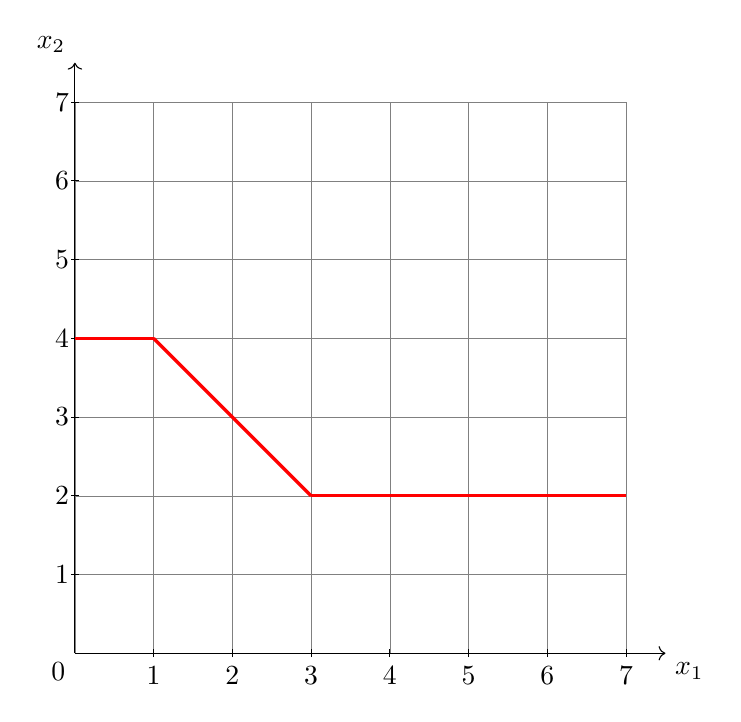
\begin{tikzpicture}
            \draw[very thin,color=gray] (0,0) grid (7,7);
            \draw[->] (0,0)--(7.5,0) node[below right] {$x_1$};
            \draw[->] (0,0)--(0,7.5) node[above left] {$x_2$};
            
            \node[below left] at (0,0) {0};

            \foreach \i in {1,...,7}
            \draw (\i,-0.05)--++(90:0.1) node[below=1mm]{\i};
            %\draw (\i,-0.05)--(\i,0.05) node[below=1mm]{\i};
            \foreach \i in {1,...,7}
            \draw (0.05,\i)--++(180:0.1) node[left=-1mm]{\i};

            \draw[domain=0:1, very thick, color=red] plot (\x, {4});
            \draw[domain=1:3, very thick, color=red] plot (\x, {-\x+5});
            \draw[domain=3:7,very thick, color=red] plot (\x, {2});
        \end{tikzpicture}
    \end{enumerate}
\end{enumerate}
\pagebreak


\end{document}